%TC:macro \cite [option:text,text]
%TC:macro \citep [option:text,text]
%TC:macro \citet [option:text,text]
%TC:envir table 0 1
%TC:envir table* 0 1
%TC:envir tabular [ignore] word
%TC:envir displaymath 0 word
%TC:envir math 0 word
%TC:envir comment 0 0
\documentclass[acmtog]{acmart}
\usepackage{graphicx}
\usepackage{listings}
\usepackage{color}
\usepackage{tikz}

\definecolor{dkgreen}{rgb}{0,0.6,0}
\definecolor{gray}{rgb}{0.5,0.5,0.5}
\definecolor{mauve}{rgb}{0.58,0,0.82}

\lstset{frame=tb,
  language=Java,
  aboveskip=3mm,
  belowskip=3mm,
  showstringspaces=false,
  columns=flexible,
  basicstyle={\small\ttfamily},
  numbers=none,
  numberstyle=\tiny\color{gray},
  keywordstyle=\color{blue},
  commentstyle=\color{dkgreen},
  stringstyle=\color{mauve},
  breaklines=true,
  breakatwhitespace=true,
  tabsize=3
}


\AtBeginDocument{%
  \providecommand\BibTeX{{%
    Bib\TeX}}}


\setcopyright{acmlicensed}
\copyrightyear{2024}
\acmYear{2024}

\citestyle{acmauthoryear}


\begin{document}

\title{Emulate ARM TrustZone on a Virtualized Xen Hypervisor}


\author{Yong Li}
\authornote{Both authors contributed equally to this research.}
\email{yonli@umass.edu}
\orcid{1234-5678-9012}
\affiliation{%
  \institution{University of Massachusetts, Amherst}
  \city{Amherst}
  \state{MA}
  \country{USA}
}

\renewcommand{\shortauthors}{Yong Li}


\begin{abstract}
\end{abstract}

\maketitle

\section{Introduction}




\subsection{Background}
Hypervisor allows multiple operating systems in parallel on the same hardware. This
technology is increasingly adopted on embedded platforms. However, the hypervisors can be
compromised by malicious agents that would lead to attacks on all the operating systems. To mitigate
such scenarios, modern hardware platforms provide trusted execution environments (TEEs) that are
protected against attacks by privileged adversary like hypervisors. However, modern hypervisors have
limited support for Trustzone (ARM’s TEE) and the potential for Trustzone to provide secure services to
virtualized systems (systems that run hypervisor) is yet untapped. The aim of this project is to build a
development environment which runs Xen hypervisor with support for ARM Trustzone. Such an
environment would enable research that enhances security of virtualized embedded systems

\subsection{Motivation}
The rise of embedded systems and their integration into critical infrastructure has necessitated enhanced security measures. Hypervisors, while powerful, are vulnerable to attacks, which can compromise all systems running on the hardware. ARM TrustZone provides a solution by creating a Trusted Execution Environment (TEE) that is isolated from the rest of the system, offering protection against privileged adversaries. This project aims to explore the potential of running Xen hypervisor with support for OP-TEE (TrustZone Software) on a QEMU-emulated ARM environment. By doing so, we can extend the benefits of TrustZone to virtualized environments, enhancing the security of embedded systems.

\subsection{Objective}
Implement a Xen hypervisor that supports OP-TEE (TrustZone Software) in a QEMU-emulated environment.
Enable research and benchmarking on the performance and security enhancements offered by TrustZone in virtualized systems.
Develop a comprehensive understanding of how virtualized systems operate with TrustZone enabled.


\section{Literature Review}
\subsection{TrustZone Technology}
ARM TrustZone is a security technology built into many ARM processors, commonly found in mobile devices and embedded systems. It creates a hardware-based separation between two "worlds": the Secure World and the Normal World.

Think of it like having two separate computers running on the same chip. The Secure World is a protected environment for sensitive tasks such as:
\begin{itemize}
  \item  Storing cryptographic keys
  \item Processing payments
  \item Running secure boot code
\end{itemize}


\subsection{Type 1 and Type 2 Hypervisors}  
Hypervisors, or Virtual Machine Monitors (VMMs), enable multiple operating systems to run simultaneously on a single physical machine. They are categorized into **Type 1** and **Type 2** based on their architecture and operation.

Type 1 Hypervisors (Bare-Metal) run directly on physical hardware, acting as the primary OS. They provide:  

Type 2 Hypervisors (Hosted) run on top of a host OS, using it for hardware management. They are ideal for development or personal use:  
 
\begin{figure}[ht]
  \centering
  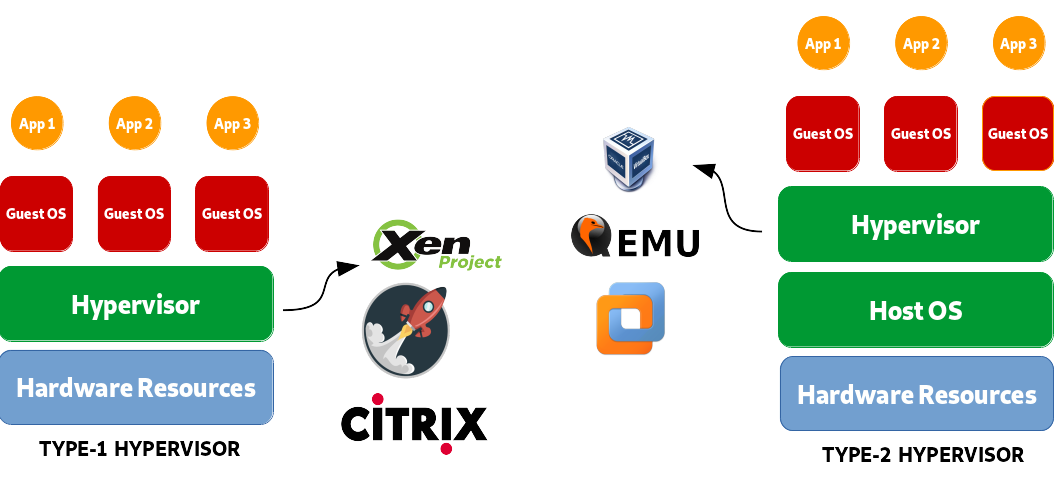
\includegraphics[width=\columnwidth]{images/hypervisor_type12.png}
  \caption{Type1 and Type2 Hypervisor}
  \label{fig:image_label}
\end{figure}

\begin{table}[h!]
\centering
\caption{Comparison of Type 1 and Type 2 Hypervisors}
\begin{tabular}{|l|l|l|}
\hline
\textbf{Feature}         & \textbf{Type 1 Hypervisor} & \textbf{Type 2 Hypervisor} \\ \hline
\textbf{Deployment}      & Runs on hardware          & Runs on a host OS          \\ \hline
\textbf{Performance}     & High                      & Moderate                   \\ \hline
\textbf{Use Case}        & Enterprise, servers       & Development, personal use  \\ \hline
\textbf{Examples}        & Xen, VMware ESXi          & VirtualBox, VMware Workstation \\ \hline
\end{tabular}
\end{table}


\section{Introduction to the Virtualization Stack}

In this section, we will explain how to enable a TrustZone-based application to run in a virtualized environment on QEMU. The process involves incrementally layering virtualization technologies, starting with the basic ARM CPU with TrustZone, then introducing the hypervisor, and finally virtualizing the ARM CPU with QEMU. Below is a high-level overview of the stack:

\begin{itemize}
    \item TrustZone Application (via OP-TEE)
    \item Linux Guest OS
    \item Hypervisor (Xen)
    \item QEMU (emulates ARM CPU)
    \item AnyCPU (host OS)
\end{itemize}

We will explore each step in detail, showing how the system is built up layer by layer.

\subsection{Step 1: Meta Machine (ARM CPU with Linux OS)}

The first step is to show the basic setup where Linux OS runs directly on an ARM CPU that supports TrustZone. TrustZone provides a hardware-based isolation mechanism, dividing the CPU into two "worlds": the secure world (TrustZone) and the non-secure world (Linux). Here, Linux directly interacts with the ARM CPU, running in the non-secure world while TrustZone applications run in the secure world. This setup represents the simplest form of running Linux with TrustZone support.

\begin{figure}[ht]
  \centering
  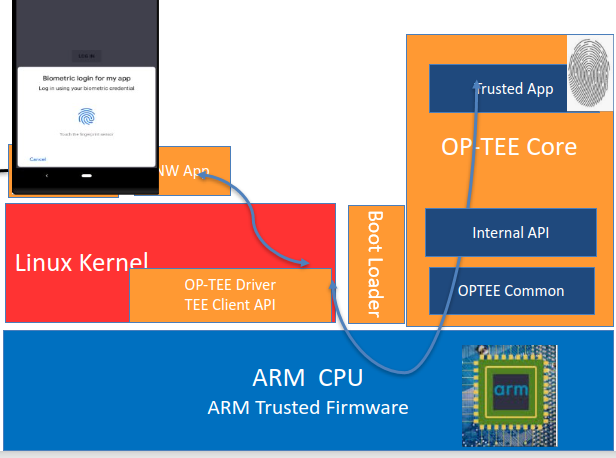
\includegraphics[width=\columnwidth]{images/env_1_bare_metal.png}
  \caption{ARM Trusted App, no virtualization}
  \label{fig:image_label}
\end{figure}



\subsection{Step 2: Introducing the Hypervisor}
The next step involves introducing a hypervisor (in this case, Xen) to the system. The hypervisor provides a layer of abstraction, allowing multiple operating systems to run concurrently on the same hardware. In this scenario, Xen is installed on the ARM CPU, and Linux is virtualized into a guest operating system. The hypervisor ensures that the guest OSes are isolated from one another and the underlying hardware. This setup enables the secure TrustZone application to run alongside the virtualized Linux OS.

In this step, we introduce the concept of a hypervisor, which is critical to enabling the virtualization of the system. The hypervisor, in this case, Xen, runs directly on the ARM CPU and acts as a layer between the hardware and the operating systems (OSes) that need to run on top of it. 

In our configuration, we utilize Xen as a Type 1 hypervisor. It runs directly on the ARM hardware, which allows it to manage the system's resources and allocate them efficiently to virtual machines (VMs). The Xen hypervisor introduces the concept of domains: 
\begin{itemize}
    \item \textbf{Domain 0 (Dom0):} This is the privileged domain that has direct access to hardware resources and manages other domains. It typically runs a Linux-based OS, which is responsible for managing virtual devices and the overall virtualization environment.
    \item \textbf{Domain U (DomU):} These are the unprivileged domains or virtual machines that run on top of Dom0. Each DomU runs its own guest operating system, which in our case is a Linux OS. DomU does not have direct access to hardware, and its interactions with the hardware must go through Dom0 or the hypervisor.
\end{itemize}

Xen ensures that these domains are isolated from one another, preventing one compromised domain from affecting the others. This isolation is a critical feature of virtualization as it allows multiple guest OSes to run safely on the same hardware, without interference.

In this configuration, Xen to virtualize the ARM CPU, enabling the ability to run multiple guest OSes on the same hardware. The host OS (AnyCPU) in the bottom layer manages the virtualization stack, while the Xen hypervisor sits directly on top of it, providing a secure and isolated environment for guest OSes.

Thus, the Xen hypervisor plays a crucial role in enabling secure, isolated, and efficient virtualization of Linux on ARM CPUs. With the introduction of Xen, we can now run multiple guest operating systems on a single ARM platform, and each of these guest OSes can leverage the security of the TrustZone, as detailed in the following steps.



\begin{figure}[ht]
  \centering
  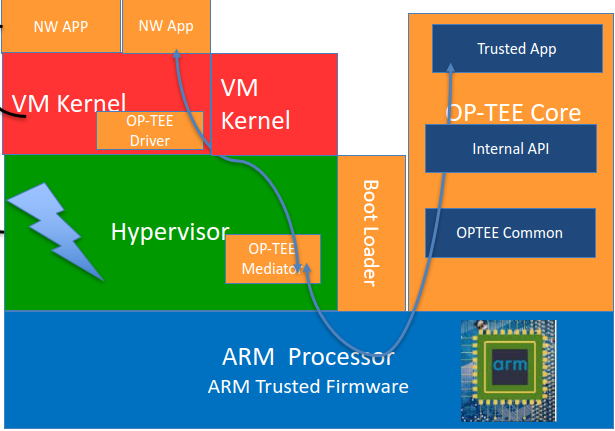
\includegraphics[width=\columnwidth]{images/env_2_add_hyperv.png}
  \caption{Linux OS is virtualized by Xen hypervisor}
  \label{fig:image_label}
\end{figure}


\subsection{Step 3: Virtualizing the ARM CPU with QEMU}
Once all steps are integrated, we arrive at the final virtualization stack. In this step, we introduce QEMU to emulate the ARM CPU on a non-ARM machine, such as an x86-based host. QEMU enables the full virtualization of the ARM architecture, allowing the Xen hypervisor to run on a virtualized ARM CPU. This configuration enables the virtualized ARM CPU to execute Linux as a guest OS. The final application in the secure world (TrustZone) runs as intended, isolated from the non-secure world.steps   This stack enables TrustZone-based applications to run on a virtualized ARM architecture, with each component providing critical functionality.

\begin{itemize}
    \item \textbf{TrustZone Application:} Runs securely in the ARM TrustZone.
    \item \textbf{Linux Guest OS:} Runs on the virtualized hardware.  
    \item \textbf{Hypervisor (Xen):} Provides the virtualization layer.  
    \item \textbf{QEMU (ARM CPU Emulated):} Emulates the ARM architecture.  
    \item \textbf{AnyCPU (Host OS):} Provides the hardware for virtualization.
\end{itemize}

\begin{figure}[ht]
  \centering
  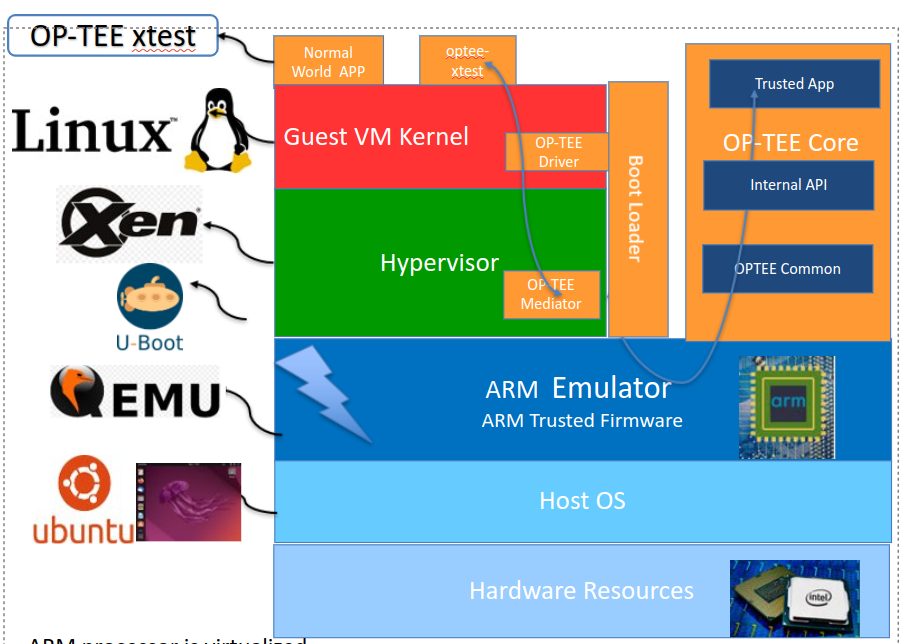
\includegraphics[width=\columnwidth]{images/optee_virtual_arch.png}
  \caption{Full Virtualization Stack. ARM Processor is virtualized by QEMU}
  \label{fig:image_label}
\end{figure}

\subsection{TrustZone within the Stack}
Within this stack, TrustZone operates at the lowest level, ensuring secure execution for applications. The Xen hypervisor virtualizes the ARM CPU, while QEMU allows the entire stack to run on any host machine. The Linux Guest OS runs in the non-secure world, while the TrustZone application interacts with the ARM CPU’s secure world. OP-TEE (Trusted Execution Environment) is used to manage the execution of these secure applications. This layered approach ensures that the secure application is isolated and protected, even in a virtualized environment.

\subsection{Recap}
To summarize the process:
\begin{itemize}
    \item We started with a bare-metal system where Linux runs directly on the ARM CPU with TrustZone.
    \item Then, we added Xen to virtualize the ARM CPU and enable multiple guest OSes.
    \item Finally, we used QEMU to emulate the ARM CPU and allow this stack to run on any hardware platform.
\end{itemize}

This layered approach demonstrates how to effectively enable TrustZone applications within a virtualized environment, providing both security and flexibility for embedded systems research.






\subsection{ARM TrustZone}
\subsection{Current Challenges}
Challenges: Highlight issues faced during setup, debugging, and modifications.

Platform: Describe QEMU as the ARM emulator and Xen as the hypervisor.
Tutorial Review: Mention tutorials used and errors encountered.

\subsection{System Architecture}



\subsection{Components}
\begin{itemize}
  \item{Hypervisor: Xen hypervisor with OP-TEE support.}
  \item{Virtual Machine Emulator: QEMU with ARM virtualization extensions.}
  \item{Operating Systems: Linux for both secure and non-secure environments.}
  \item{Benchmarks: xtest for performance evaluation.}
\end{itemize}


\subsection{xen}
Xen offers two types of virtualization: paravirtualization and full virtualization.

In paravirtualization, the virtualized operating system operates on a tweaked version of the OS. As a result, the tweaked operating system becomes aware that it is virtualized. This permits more efficient interaction between the OS and the physical hardware since the hardware devices are addressed directly. However, the fact that the functionality of paravirtualization relies on modified guest OS is a downside since most vendors do not provide it.

Xen also offers full virtualization, a mode where all virtualization extensions require the CPU's support. Here, the unmodified operating systems can efficiently instruct the hardware because of this support. Full virtualization often comes with performance drawbacks because complete emulation usually requires more processing resources and overhead resources from the hypervisor.


\subsection{Role of a Hypervisor}
We can’t allow VMs to call OP-TEE directly. There are multiple
consideration concerning both virtualization mechanism and
security:
I VM does not know physical addresses of own buffers
I OP-TEE needs to know when VM is created or destroyed
I OP-TEE needs to know which VM calls it
I We need to ensure that VM does not try to provide OP-TEE
with memory reference to another VM’s memory

\subsection{ Hypervisor Intermediate Physical Addresses}
We all know the idea of virtual memory: Memory Management
Unit (MMU) translates virtual memory addresses to real physical
ones:
VA PA
MMU
In most cases, when virtualization is used, we add a second stage
of MMU translation and new type of address: Intermediate
Physical Address (IPA):
VA IPA
MMU 1st stage
PA
MMU 2nd stage
Virtual machines manages translation tables for the first stage and
believes that it is working with real physical memory. But in reality
it lives in virtual address space. Hypervisor manages second stage
translation which translates IPAs to PAs.
This approach allows hypervisor to manage address spaces of VMs
in the same way as OS manages address spaces for processes

So, virtual machine sees only IPA and don’t know real address of
it’s memory pages. On other hand, OP-TEE know nothing about
IPAs and always expects real physical addresses to be passed from
Normal World.
This is where hypervisor steps is. It traps all calls from VMs to
OP-TEE and translates IPAs to PAs in all requests. In the
meantime it also ensures that all memory pages in question belong
to the VM. (Also, ensures that those memory pages will stay in
memory for the whole duration).
VM
Hypervisor: translate addresses, add VMID
SMC (trapped) or HVC
OP-TEE


OP-TEE need to track life cycle of VMs. So it provides two special
calls: 
\begin{itemize}
  \item \texttt{OPTEE\_SMC\_VM\_CREATED VMID}
  \item \texttt{OPTEE\_SMC\_VM\_DESTROYED VMID}
\end{itemize}
Hypervisor informs OP-TEE about VM creation or destruction by
issuing above SMCs
\subsection{OPTEE Virtualization Support (Mediator in Hypervisor)}
OP-TEE have experimental virtualization support. This is when one OP-TEE instance can run TAs from multiple virtual machines. OP-TEE isolates all VM-related states, so one VM can’t affect another in any way.

With virtualization support enabled, OP-TEE will rely on a hypervisor, because only the hypervisor knows which VM is calling OP-TEE. Also, naturally the hypervisor should inform OP-TEE about creation and destruction of VMs. Besides, in almost all cases, hypervisor enables two-stage MMU translation, so VMs does not see real physical address of memory, instead they work with intermediate physical addresses (IPAs). On other hand OP-TEE can’t translate IPA to PA, so this is a hypervisor’s responsibility to do this kind of translation. So, hypervisor should include a component that knows about OP-TEE protocol internals and can do this translation. We call this component “TEE mediator” and right now only XEN hypervisor have OP-TEE mediator.

Compile XEN with Optee Support. To enable OP-TEE support:

Navigate to the Xen source directory.
Run the make menuconfig command to access Xen’s configuration menu.
Enable the OPTEE option and ensure that the TEE option is also enabled.
Save and exit the menuconfig tool.
Once you enable it, Xen will compile with OP-TEE support.

XEN Interactive MenuConfig path for OP-TEE: 
Xen/arm 4.18.0 configuration -> Architecture Features -> TEE mediators -> Enable OP-TEE mediator (UNSUPPORTED)

\begin{figure}[ht]
  \centering
  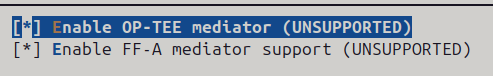
\includegraphics[width=\columnwidth]{images/optee_xen_support.png}
  \caption{XEN MenuConfig for OPTEE}
  \label{fig:image_label}
\end{figure}

Xen Non-Interactive (Command-Line) Configuration:
\begin{lstlisting}[language=make, caption=Enable OP-TEE Support in Xen]  
# Xen configuration file path  
/home/ryan/Projects/xenonarm/optee3/build/../xen/xen/.config  

# Enable TEE mediators  
CONFIG_TEE=y       # Enable Trusted Execution Environment (TEE) support  
CONFIG_OPTEE=y     # Enable OP-TEE mediator support in Xen  
\end{lstlisting}  



\subsection{OP-TEE Linux Kernel Support}
The OP-TEE driver in the guest VM kernel is essential for enabling secure communication between the guest operating system and the Trusted Execution Environment (TEE) provided by OP-TEE. In a virtualized environment, guest VMs rely on the hypervisor to manage hardware resources, but direct access to TrustZone features is not inherently available to these VMs. The OP-TEE driver acts as an intermediary, allowing guest applications to issue secure requests to OP-TEE. This integration ensures that security-critical operations, such as cryptographic computations and secure storage, can be performed in the TEE without exposing sensitive data to the untrusted hypervisor or other guest VMs. Furthermore, the driver abstracts the complexity of managing TrustZone interactions, enabling seamless use of OP-TEE services within the virtualized ecosystem, thus enhancing the security capabilities of the guest VM.

To enable the OP-TEE driver in the guest VM kernel, the configuration must be set within the Linux kernel menuconfig tool. The specific path to access and configure this driver is:
.config - Linux/x86 6.1.18 Kernel Configuration -> Device Drivers -> Trusted Execution Environment Support

The following commands and configurations are applied via the command line:
\begin{lstlisting}[language=make, caption=Enabling OP-TEE in the Linux Kernel Configuration]
  cd $WORK_DIR/linux-6.1.18/
  make ARCH=arm64 CROSS_COMPILE=aarch64-linux-gnu- defconfig
  
  # Relevant kernel configuration options
  .config
      CONFIG_XEN_DOM0=y     # Enable Xen support for Domain 0
      CONFIG_XEN=y          # Enable Xen support in the kernel
      
      CONFIG_TEE=y          # Enable Trusted Execution Environment (TEE) support
      CONFIG_OPTEE=y        # Enable OP-TEE support
  \end{lstlisting}


\section{Development Environment Setup / Implementation}
\subsection{01 install qemu for arm64}
\subsection{02 build install busybox}
\subsection{03 build install linux}
\subsection{04 verify busybox linux qemu}
\subsection{05 build install u-boot}
\subsection{06 build install xen}
\subsection{06 build install xen with virtu}
\subsection{07 disable pl061 on dtb}
\subsection{08 verify xen with linux as dom0}
\subsection{09 verify xen linux busybox on qemu with u-boot}
\subsection{10 verify dom0 domu on qemu}



\section{Results and Discussion}
\subsection{Environment Validation}
Screenshots or logs demonstrating Xen running successfully on QEMU.
Errors fixed in tutorials or configuration.

\subsection{TrustZone Functionality}
Logs or screenshots confirming OP-TEE integration.
Issues resolved during TrustZone setup.

\subsection{Benchmark Performance}
Results of xtest benchmarks in single and multiple OS environments.
Comparison of performance with and without TrustZone.

\subsection{Analysis}
Discussion of findings and their implications for enhancing security in virtualized embedded systems.


\section{Conclusion}



\bibliographystyle{ACM-Reference-Format}
\bibliography{references}

\end{document}
\endinput